\subsubsection{Move}

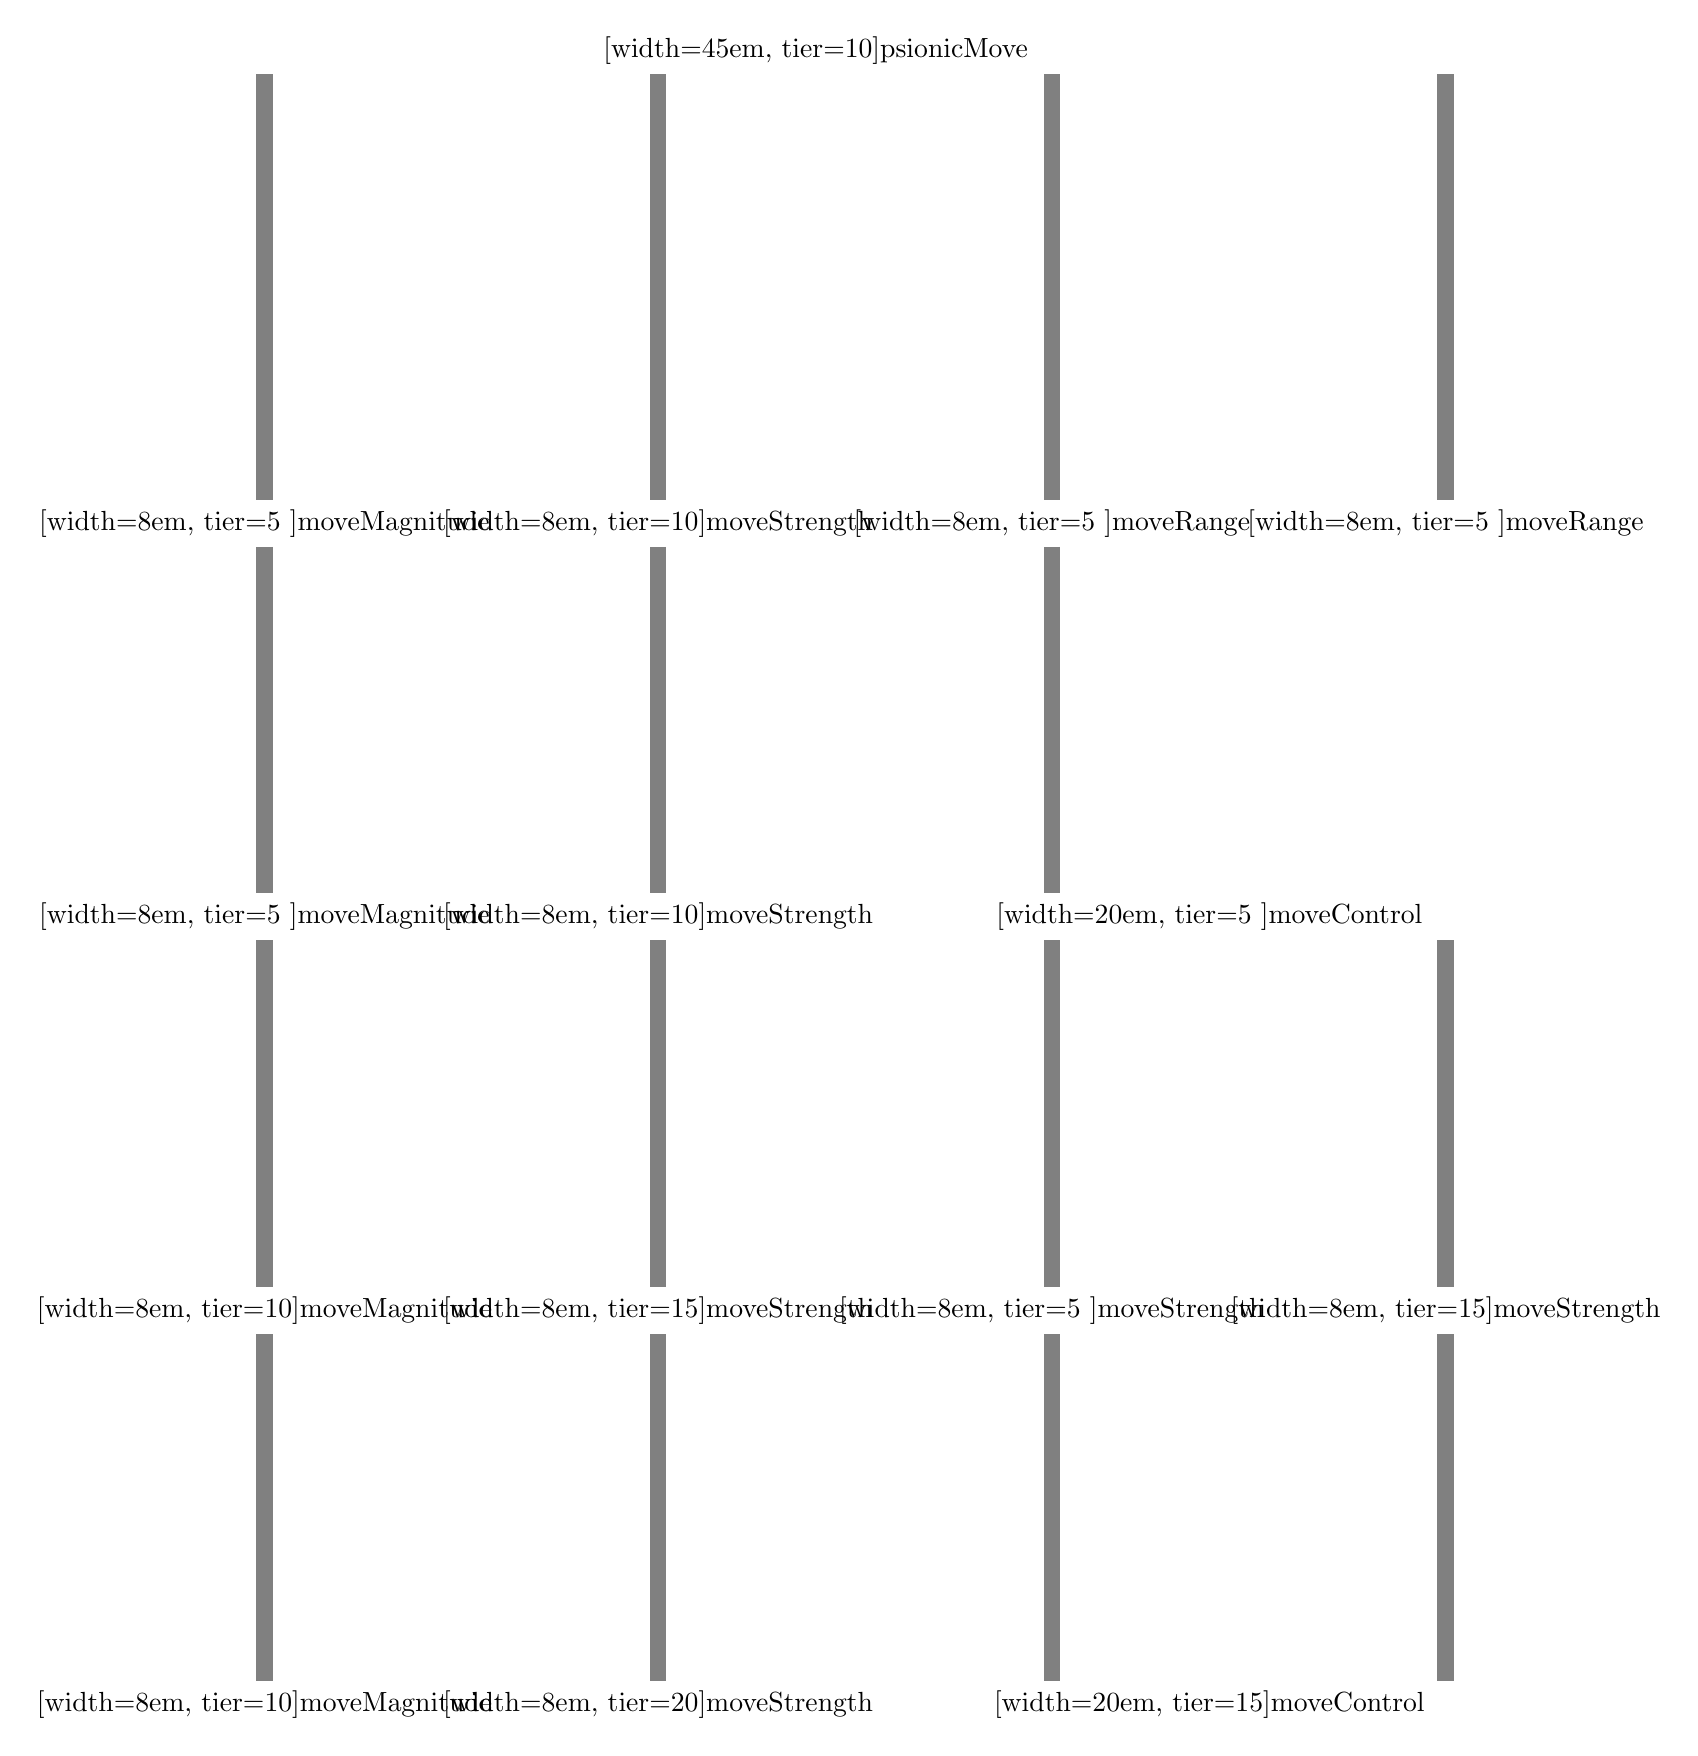
\begin{tikzpicture}
    \draw (-13,   6) node(pr){\TalentBox[width=45em, tier=10]{psionicMove}};
    \draw (-20,   0) node(aa){\TalentBox[width=8em,  tier=5 ]{moveMagnitude}}
          (-15,   0) node(ab){\TalentBox[width=8em,  tier=10]{moveStrength}}
          (-10,   0) node(ac){\TalentBox[width=8em,  tier=5 ]{moveRange}}
          ( -5,   0) node(ad){\TalentBox[width=8em,  tier=5 ]{moveRange}}
          (-20,  -5) node(ba){\TalentBox[width=8em,  tier=5 ]{moveMagnitude}}
          (-15,  -5) node(bb){\TalentBox[width=8em,  tier=10]{moveStrength}}
          ( -8,  -5) node(bd){\TalentBox[width=20em, tier=5 ]{moveControl}}
          (-20, -10) node(ca){\TalentBox[width=8em,  tier=10]{moveMagnitude}}
          (-15, -10) node(cb){\TalentBox[width=8em,  tier=15]{moveStrength}}
          (-10, -10) node(cc){\TalentBox[width=8em,  tier=5 ]{moveStrength}}
          ( -5, -10) node(cd){\TalentBox[width=8em,  tier=15]{moveStrength}}
          (-20, -15) node(da){\TalentBox[width=8em,  tier=10]{moveMagnitude}}
          (-15, -15) node(db){\TalentBox[width=8em,  tier=20]{moveStrength}}
          ( -8, -15) node(dd){\TalentBox[width=20em, tier=15]{moveControl}}
    ;

    \tikzstyle{bar}=[gray,-,>=stealth, line width=6pt]

    \draw [bar] (aa) -- (aa |- pr.south);
    \draw [bar] (ab) -- (ab |- pr.south);
    \draw [bar] (ac) -- (ac |- pr.south);
    \draw [bar] (ad) -- (ad |- pr.south);
    \draw [bar] (aa) edge (ba);
    \draw [bar] (ab) edge (bb);
    \draw [bar] (ac) -- (ac |- bd.north);

    \draw [bar] (ba) edge (ca);
    \draw [bar] (bb) edge (cb);

    \draw [bar] (cc) -- (cc |- bd.south);
    \draw [bar] (cd) -- (cd |- bd.south);
    \draw [bar] (ca) edge (da);
    \draw [bar] (cb) edge (db);
    \draw [bar] (cc) -- (cc |- dd.north);
    \draw [bar] (cd) -- (cd |- dd.north);
\end{tikzpicture}
